\documentclass[12pt]{article} 
\usepackage[utf8]{inputenc}
\usepackage[spanish,es-tabla]{babel}
\usepackage{amsmath, amssymb}
\usepackage{graphicx}
\usepackage[margin=2.5cm]{geometry}
\usepackage{subcaption}
\usepackage{setspace}
\usepackage{xcolor} 
\usepackage{titlesec} 
\usepackage{booktabs}

% --- CONFIGURACIÓN DE TIKZ (Ordenada y unificada) ---
\usepackage{tikz}
\usetikzlibrary{arrows.meta, positioning}

% --- CONFIGURACIÓN DE CITAS ---
\usepackage[style=ieee, backend=biber]{biblatex}
\addbibresource{ref_mace.bib} 

% --- HYPERREF SIEMPRE AL FINAL DEL PREÁMBULO ---
\usepackage{hyperref}      
\hypersetup{
    hidelinks
}

\begin{document}

% \section{Cálculo ab initio sobre el dímero de Hemozoina ($\beta\text{-hematina}$)}

\section{Cálculo ab initio de los parámetros kMC}

En este trabajo se toma como referencia la estructura reportada por Becker et al. \cite{becker2016bhematin}, la cual está constituida por dos monómeros de ferriprotoporfirina IX. Este dímero se asume convencionalmente como la unidad de crecimiento (GU) fundamental, caracterizada por un enlace recíproco de tipo $\mu\text{-propionato}$ (ver Figura \ref{subfig:mu_propionato}). Sin embargo, en el trabajo de Ma et al. \cite{nonclassical2025ma} se propone que la GU más estable corresponde a un arreglo por apilamiento $\pi\text{-}\pi$. Con el propósito de seguir este modelo, se adaptó la estructura original de Becker empleando sus coordenadas cristalográficas para construir el dímero de apilamiento $\pi\text{-}\pi$ (ver Figura \ref{subfig:pi_pi}).  

\begin{figure}[htbp]
    \centering
    % --- PRIMERA FIGURA (Izquierda) ---
    \begin{subfigure}[b]{0.48\textwidth}
        \centering
        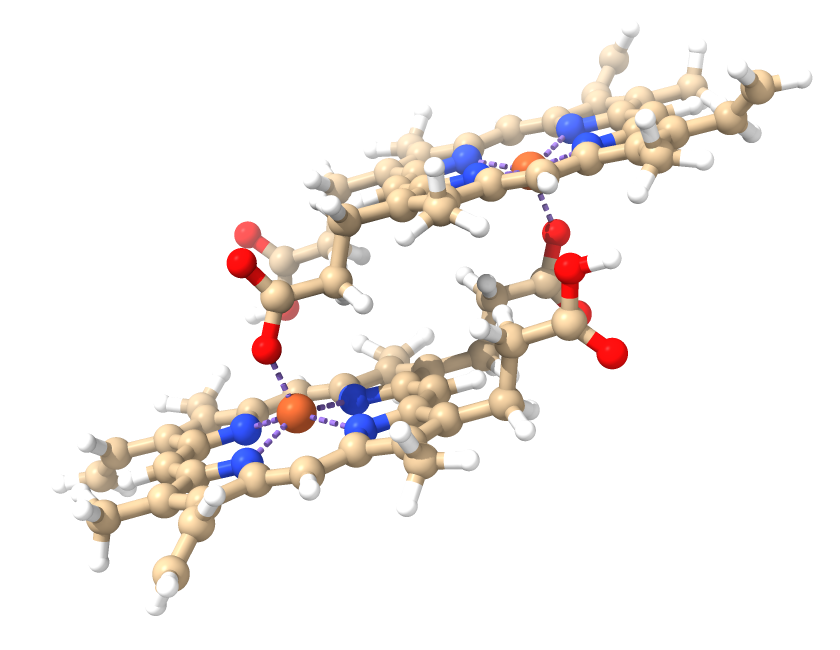
\includegraphics[width=\textwidth]{figures/GU_mupr.png} 
        \caption{Unidad de crecimiento de tipo $\mu\text{-propionato}$}
        \label{subfig:mu_propionato}
    \end{subfigure}
    \hfill 
    % --- SEGUNDA FIGURA (Derecha) ---
    \begin{subfigure}[b]{0.48\textwidth}
        \centering
        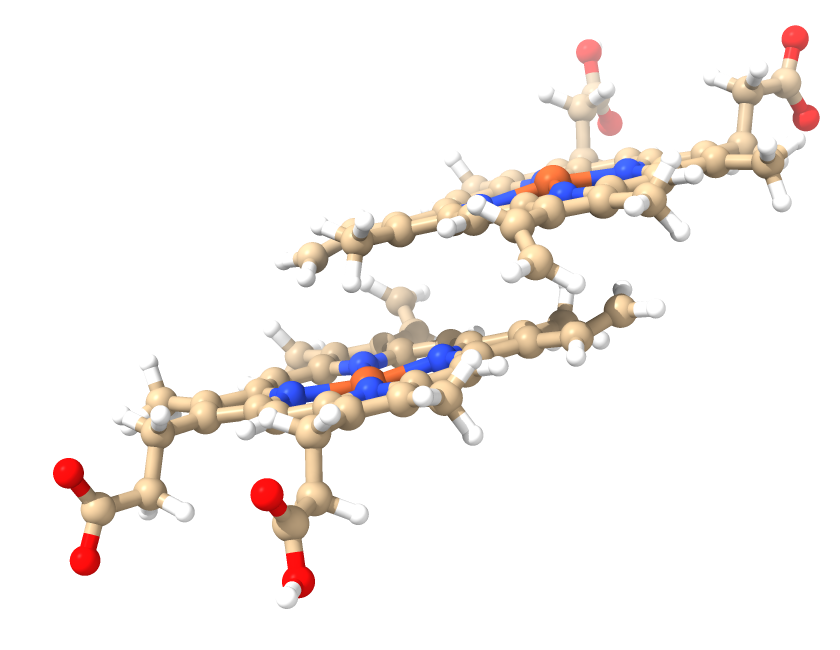
\includegraphics[width=\textwidth]{figures/hemozoin.png} 
        \caption{Unidad de crecimiento de tipo $\pi\text{-}\pi$}
        \label{subfig:pi_pi}
    \end{subfigure}
    
    \caption{Modelos de las unidades de crecimiento de la hemozoína.}
    \label{fig:unidades_crecimiento}
\end{figure}

Para obtener la estructura final empleada en los cálculos energéticos, se sometió al dímero de apilamiento $\pi\text{-}\pi$ a un proceso de relajación geométrica. Para ello, se utilizó el software ASE (Atomic Simulation Environment) en combinación con el calculador MACE, un potencial interatómico basado en Machine Learning (MLIP) \cite{batatia2023mace}.

\subsection{MLIPs: MACE}
\label{subsec:metodo_mace}

El estudio de sistemas moleculares complejos en física del estado sólido y química computacional requiere describir con alta precisión las interacciones atómicas. Así es posible determinar estructuras de mínima energía y trayectorias dinámicas. Tradicionalmente, niveles altos de precisión se alcanzan mediante métodos \textit{ab initio} basados en la teoría del funcional de densidad (DFT). Sin embargo, el costo computacional del DFT escala de forma cúbica o superior con respecto al número de electrones del sistema ($\mathcal{O}(N^3)$) \cite{capelle2006birds}. Esto limita en la práctica la exploración de sistemas de gran tamaño o simulaciones de dinámica molecular en escalas de tiempo macroscópicas.

Como alternativa para superar este cuello de botella computacional, en los últimos años han emergido los potenciales interatómicos basados en Machine Learning (MLIPs, por sus siglas en inglés). Los MLIPs actúan como interpoladores de alta fidelidad, se entrenan a partir de un conjunto de datos previos calculados con metodologías \textit{ab initio} (como DFT) para aprender la superficie de energía potencial del sistema. Una vez entrenado, el modelo es capaz de predecir energías y fuerzas atómicas con una precisión cercana a la de los métodos cuánticos primarios, pero con un costo computacional drásticamente menor, permitiendo un escalamiento lineal $\mathcal{O}(N)$ comparable al de los campos de fuerza clásicos \cite{batatia2023mace}.

Dentro de los MLIPs de última generación, MACE (Multi-Layer Atomic Cluster Expansion) destaca por el uso de redes neuronales de paso de mensajes equivariantes (MPNN) \cite{batatia2023mace, batatia2026macepolar}. A diferencia de los potenciales invariantes tradicionales, MACE preserva explícitamente la simetría rotacional y traslacional del espacio tridimensional mediante el uso de armónicos esféricos para describir los entornos atómicos. Esto le permite capturar interacciones físicas de largo alcance y correlaciones de muchos cuerpos (\textit{higher-order many-body interactions}) con un número significativamente menor de parámetros y datos de entrenamiento.

En este trabajo, MACE en su modelo \textit{polar} se establece como el motor de cálculo fundamental. Este modelo permite el calculo de energías de grandes sistemas como lo es la GU de hemozina (con 148 átomos por cada GU) incorporando interacciones electrostáticas con un bajo coste computacional y una alta precisión \cite{batatia2026macepolar}. El modelo \textit{polar} en sus versiones \textsc{medium} y \textsc{large} fue entrenado empleando la base de datos OMol25 \cite{ batatia2026macepolar,omol2025}, esta base de datos corresponde a cálculos realizados con el funcional $\omega\text{B97M-V}$ el cual captura interacciones electrostáticas de largo alcance \cite{mardirossian2016wb97m}. 

La arquitectura de MACE-\textit{polar} se divide en dos componentes principales: la predicción de energía en entornos locales ($E_{\text{local}}$) mediante MACE como MPNN \cite{batatia2023mace} y la predicción de la energía no local y electrostática ($E_{\text{non-local}} + E_{\text{electrostatic}}$) mediante una construcción de la densidad de espín-carga en un modelo de expansión multipolar \cite{batatia2026macepolar}. Ambos componentes son procesos basados en Machine Learning: el primero predice la energía del estado base de una configuración atómica al suponer los sistemas atómicos como grafos cuyos nodos vecinos pueden interactuar a través de un proceso denominado como construcción e intercambio de mensaje como se ve en la figura \ref{subfig:diagrama_mace_local}. Esta construcción de mensaje se produce como una expansión en una base radial aprendida (empleando las funciones de Bessel) y los armónicos esféricos. Los coeficientes de la expansión mezclan las características de cada nodo que participa del intercambio. A través de un proceso de lectura en el cual se emplea un perceptrón multicapa (MLP) cada configuración atómica predice una energía local \cite{batatia2023mace}. El segundo componente predice la densidad de espín-carga de la configuración atómica mediante una expansión multipolar que emplea orbitales de tipo Gaussiano, los coeficientes de la expansión se predicen mediante un MLP de las características de cada nodo. Estos coeficientes se emplean para la predicción de las energías no locales y electrostáticas como se muestra en la figura \ref{subfig:diagrama_mace_polar_lr}, la primera a través de una sucesión de MLP sobre las características de los nodos de la configuración y la segunda integrando la energía de Hartree y el potencial externo aplicado \cite{batatia2026macepolar}.

\begin{figure}[htbp]
    \centering
    % =========================================================================
    % SUBFIGURE A: MACE (Message Passing)
    % =========================================================================
    \begin{subfigure}[b]{0.49\textwidth}
        \centering
        \begin{tikzpicture}[
            scale=0.75,                        % Escala el lienzo para el subplot izquierdo
            every node/.style={scale=0.75},     % Escala el texto de forma uniforme
            node distance=0.9cm,
            auto,
            block/.style={
                rectangle, 
                draw=black, 
                thick,
                fill=gray!10, 
                text width=7.0cm,              % Ancho adaptado para la columna izquierda
                text centered, 
                rounded corners, 
                minimum height=1.2cm,
                font=\small
            },
            line/.style={
                draw, 
                -latex, 
                thick
            }
        ]
            % --- NODOS MACE ---
            \node [block, fill=blue!5] (input) {
                \textbf{Entrada: Configuración Atómica} \\ 
                Coordenadas cartesianas $\vec{r}_i$ y números atómicos $Z_i$ para la conformación de $\vec{\sigma}_i$
            };
            
            \node [block, below=of input] (embedding) {
                \textbf{1. Bloque de Embedding } \\ 
                \textbf{Atómico:} $Z_i \rightarrow h_i^{(0)}$ \\ \textbf{Geométrico:} Radial y Angular $Y_l^m(\hat{r}_{ij})$
            };
            
            \node [block, below=of embedding] (messages) {
                \textbf{2. Construcción de Mensajes} \\ 
                Combinación densa de bases para formar los coeficientes $B_{i, \eta \nu kLM}$ del mensaje $m_i^{(t)}$
            };
            
            \node [block, below=of messages] (update) {
                \textbf{3. Actualización de Estados} \\ 
                Actualización del embedding invariante: $h_i^{(t+1)} = W(m_i^{(t)},h_i^{(t)})$
            };
            
            \node [block, below=of update] (readout) {
                \textbf{4. Lectura Local} \\ 
                Mapeo via MLP para predecir la energía del sitio local: $E_i = \mathcal{R}(h_i^{(0)},\dots,h_i^{(T)})$
            };
            
            \node [block, below=of readout, fill=green!5] (output) {
                \textbf{Salida: Energía Total MACE} \\ 
                Predicción por suma directa: $E_{\text{local}} = \sum_{i} E_i$
            };
            
            % --- ENLACES MACE ---
            \path [line] (input) -- (embedding);
            \path [line] (embedding) -- (messages);
            \path [line] (update) -- (readout);
            \path [line] (readout) -- (output);
    
            \path [line] (messages.west) to[out=180, in=180, looseness=1.0] node[left, pos=0.5, font=\scriptsize] {Iteración $t$} (update.west);
            \path [line] (update.east) to[out=0, in=0, looseness=1.0] (messages.east);
        \end{tikzpicture}
        \caption{Algoritmo MACE (Interacciones locales).}
        \label{subfig:diagrama_mace_local}
    \end{subfigure}
    \hfill % Fuerza la separación horizontal máxima entre ambos subplots
    %=========================================================================
    % SUBFIGURE B: MACE-POLAR (Long-Range / Electrostatic)
    % =========================================================================
    \begin{subfigure}[b]{0.49\textwidth}
        \centering
        \begin{tikzpicture}[
            scale=0.75,                        % Escala el lienzo para el subplot derecho
            every node/.style={scale=0.75},     % Escala el texto de forma uniforme
            node distance=0.9cm,
            auto,
            block/.style={
                rectangle, 
                draw=black, 
                thick,
                fill=gray!10, 
                text width=7.0cm,              % Ancho adaptado para la columna derecha
                text centered, 
                rounded corners, 
                minimum height=1.2cm,
                font=\small
            },
            line/.style={
                draw, 
                -latex, 
                thick
            }
        ]
            % --- NODOS MACE-POLAR ---
            \node [block, fill=blue!5] (input_p) {
                \textbf{Entrada: Restricciones Globales} \\ 
                Posiciones Atómicas, Carga Total $Q$ y Espín Total $S$
            };
            
            \node [block, below=of input_p] (init_p) {
                \textbf{1. Inicialización de Multipolos} \\ 
                Predicción de multipolos iniciales $\tilde{p}_{i,lm}^{(0)}$ y funciones de Fukui $f_i^{(0)}$ desde MACE
            };
            
            \node [block, below=of init_p] (poisson_p) {
                \textbf{2. Solución de Poisson Global} \\ 
                Construcción de la densidad $\rho(r)$ y convolución con el núcleo de Coulomb para obtener $v(r)$
            };
            
            \node [block, below=of poisson_p] (induction_p) {
                \textbf{3. Inducción y Equilibrio} \\ 
                Refinamiento de multipolos $p_{i,lm}^{(u)}$ + Normalización de Fukui para conservar $Q$ y $S$
            };
            
            \node [block, below=of induction_p] (energy_p) {
                \textbf{4. Cálculos Energéticos} \\ 
                \textbf{Electrostática:} $E = \frac{1}{2} \int \rho v$ \\ \textbf{No-Local:} $E = \text{MLP}(\vec{h}^{(T)})$
            };
            
            \node [block, below=of energy_p, fill=green!5] (output_p) {
                \textbf{Salida: Energía No-Local Total} \\ 
                $E_{\text{LR}} = E_{\text{electrostatic}} + E_{\text{non-local}}$
            };
            
            % --- ENLACES MACE-POLAR ---
            \path [line] (input_p) -- (init_p);
            \path [line] (init_p) -- (poisson_p);
            \path [line] (induction_p) -- (energy_p);
            \path [line] (energy_p) -- (output_p);
            
            \path [line] (poisson_p.west) to[out=180, in=180, looseness=1.0]  (induction_p.west);
            \path [line] (induction_p.east) to[out=0, in=0, looseness=1.0] node[right, pos=0.5, font=\scriptsize] {Inducción $u$}(poisson_p.east);
        \end{tikzpicture}
        \caption{MACE-Polar (Efectos de largo alcance).}
        \label{subfig:diagrama_mace_polar_lr}
    \end{subfigure}

    \caption{Arquitectura integrada de MACE y MACE-Polar para el cálculo de propiedades moleculares.}
    \label{fig:arquitectura_mace_completa}
\end{figure}

\subsection{Relajación de la Estructura}

Para la determinación de la estructura cristalina óptima, se tomó como configuración inicial el dímero con apilamiento $\pi\text{-}\pi$ obtenido a partir de la GU reportada por Becker et al. \cite{becker2016bhematin}, ilustrada en la Figura \ref{subfig:pi_pi}. Los parámetros de red experimentales de dicha referencia se utilizaron para construir la celda unitaria inicial, aplicando condiciones periódicas de frontera (PBC) en las tres dimensiones. Las interacciones interatómicas se modelaron empleando el modelo \textit{polar-1-l} de MACE.

El proceso de relajación estructural se llevó a cabo en dos etapas consecutivas utilizando el entorno ASE. En la primera etapa, se realizó una optimización geométrica exclusiva de la celda manteniendo las posiciones atómicas fijas en coordenadas fraccionarias; para ello, se empleó el formalismo de deformación homogénea mediante la herramienta \texttt{StrainFilter} acoplada al algoritmo Cuasi-Newton de memoria limitada L-BFGS, utilizando un criterio de convergencia en las fuerzas de $F_{\text{max}} = 0.05$ \text{ eV/\AA}. En la segunda etapa, se procedió con una relajación conjunta y acoplada de las coordenadas atómicas y los vectores de la celda (relajación de celda variable). Esta fase se ejecutó mediante el algoritmo \texttt{FrechetCellFilter} en el espacio exponencial y el optimizador L-BFGS, bajo un criterio de convergencia más estricto de $F_{\text{max}} = 0.01$ \text{ eV/\AA}.

Como resultado de este protocolo de optimización, se determinaron los parámetros de red calculados para el estado base del cristal: $a = 16.218$ \text{\AA}, $b = 24.214$ \text{\AA}, $c = 7.758$ \text{\AA}, $\alpha = 135.440^\circ$, $\beta = 120.054^\circ$ y $\gamma = 37.008^\circ$, para una comparación con los parámetros iniciales ver la tabla \ref{tab:parametros_red}.

% =========================================================================
% SECCIÓN OPCIONAL: Sugerencia de tabla para comparar con el experimento
% =========================================================================
\begin{table}[htbp]
\centering
\caption{Comparación de los parámetros de red determinados mediante el campo de fuerza por Becker et al. \cite{becker2016bhematin} frente a los valores optimizados mediante el potencial MACE (\textit{polar-1-l}).}
\label{tab:parametros_red}
\begin{tabular}{lcc}
\toprule
\textbf{Parámetro} & \textbf{Previo \cite{becker2016bhematin}} & \textbf{Optimizado (Este trabajo)} \\
\midrule
$a$ (\AA)       & $16.636$ & $16.218$ \\
$b$ (\AA)       & $24.846$ & $24.214$ \\
$c$ (\AA)       & $7.990$ & $7.758$  \\
$\alpha$ ($^\circ$) & $135.205$ & $135.440$ \\
$\beta$ ($^\circ$)  & $119.553$ & $120.054$ \\
$\gamma$ ($^\circ$) & $36.874$ & $37.008$  \\
\bottomrule
\end{tabular}
\end{table}

\subsection{Cálculos de Energía de Enlace ($E_{\text{pb}}$)}
\label{subsec:calculos_epb}

Para la determinación de las energías de enlace ($E_{\text{pb}}$), se tomó como estado de referencia la GU relajada bajo condiciones periódicas de frontera (PBC). Debido a la naturaleza intrínseca del cálculo de interacciones aisladas, es necesario desactivar las PBC y realizar una re-optimización geométrica en el vacío. 

Con el propósito de evitar artefactos estructurales artificiales en el vacío, tales como el colapso de los grupos carboxilo terminales que originalmente se coordinan con los centros de hierro de las GU adyacentes, se procedió a saturar los átomos de oxígeno externos mediante la adición de átomos de hidrógeno (ver la figura \ref{fig:H-extra}). Físicamente, se puede aproximar a la presencia de una solución.

\begin{figure}[htbp]
    \centering
    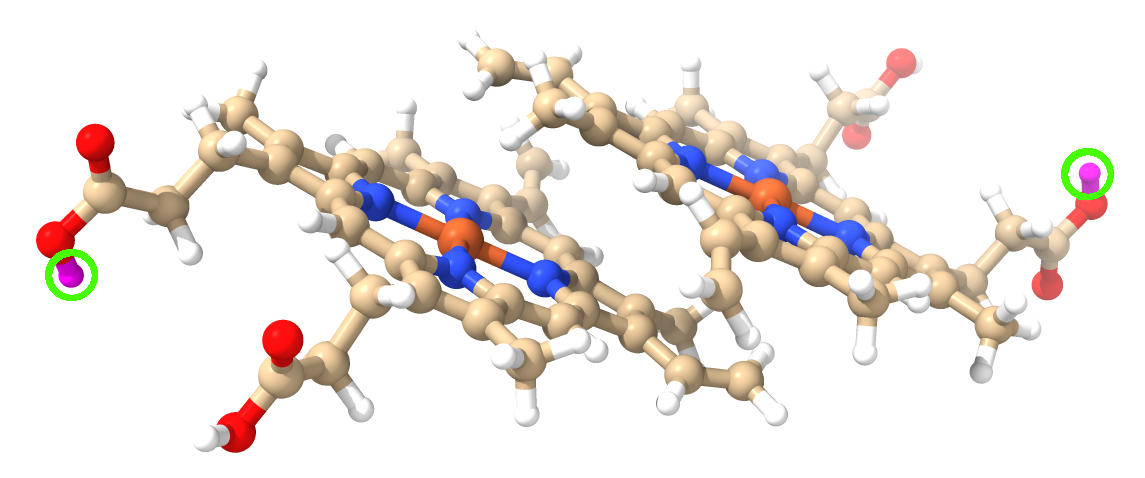
\includegraphics[width=0.8\linewidth]{figures/H_extra.png}
    \caption{Estructura con adición de Hidrógenos para la estabilización de la geometría.}
    \label{fig:H-extra}
\end{figure}

El protocolo de relajación de las GU modificadas se ejecutó en dos etapas sucesivas mediante el algoritmo LBFGS:
\begin{enumerate}
    \item \textbf{Optimización parcial:} Se mantuvieron fijos todos los átomos de la GU original, permitiendo la libre movilidad únicamente de los hidrógenos añadidos para optimizar las distancias de enlace de los grupos hidroxilo.
    \item \textbf{Optimización global:} Se liberaron todos los grados de libertad del sistema hasta alcanzar la convergencia geométrica total.
\end{enumerate}

Para aislar y contrarrestar la contribución energética de los hidrógenos extra en el balance termodinámico, se optimizó de manera independiente una molécula de $\text{H}_2$ en el vacío bajo el mismo nivel de teoría. Así, para la dirección del enlace $\mu\text{-propionato}$, donde se remueven los hidrógenos correspondientes para evaluar la coordinación metal-ligando, la energía se computa como:
\begin{equation*}
    E_{\mu\text{-Pr}} = E_{\text{dim}} + E_{\text{H}_2} - 2E_{\text{GU}}
\end{equation*}
Mientras que para las componentes restantes, donde no se requiere la remoción de los agentes de saturación, la energía de interacción se define directamente mediante la diferencia:
\begin{equation*}
    E_{\text{pb}} = E_{\text{dim}} - 2E_{\text{GU}}
\end{equation*}

Los resultados energéticos obtenidos a través del calculador MACE, junto con las energías de interacción molecular para cada orientación cristalográfica y sus respectivos promedios de par, se consolidan en la tabla \ref{tab:energias_hemozoin}.

\begin{table}[htbp]
    \centering
    \caption{Energías totales calculadas de enlace $E_{\text{pb}}$ determinadas con MACE}
    \label{tab:energias_hemozoin}
    \small
    \begin{tabular}{lc}
        \hline
        \textbf{Configuración / Parámetro} & \textbf{Energía (eV)} \\ \hline
        Energía de un monómero aislado relajado ($E_{\text{GU}}$) & $-168\,634.0454$ \\ [1ex]
        \textbf{Energías de Enlace ($E_{\text{pb}}$)} & \\
        \quad Dirección $\mu$-propionato & $-0.7609$ \\
        \quad Dirección Enlace de Hidrógeno (H-Bond) & $-0.7420$ \\
        \quad Dirección P-P & $-2.1994$ \\ [1ex]
        \textbf{Promedios de Pares Intermoleculares} & \\
        \quad Promedio $\mu$-propionato \,+\, H-Bond & $-0.7514$ \\
        \quad Promedio $\mu$-propionato \,+\, P-P & $-1.4801$ \\
        \quad Promedio H-Bond \,+\, P-P & $-1.4707$ \\ [1ex]
        \hline
        \textbf{PROMEDIO TOTAL DE ENLACE} & $\mathbf{-1.2341}$ \\ \hline
    \end{tabular}
\end{table}

\printbibliography

\end{document}
